\documentclass[11pt, a4paper]{article}
\usepackage{pdfpages}
\usepackage{parallel}
\usepackage[T2A]{fontenc}
\usepackage{ucs}
\usepackage[utf8x]{inputenc}
\usepackage[polish,english,russian]{babel}
\usepackage{hyperref}
\usepackage{rotating}
\usepackage[inner=2cm,top=1.8cm,outer=2cm,bottom=2.3cm,nohead]{geometry}
\usepackage{listings}
\usepackage{graphicx}
\usepackage{wrapfig}
\usepackage{longtable}
\usepackage{indentfirst}
\usepackage{array}
\usepackage{tikzsymbols}
\usepackage{soul}
\usepackage[ruled,vlined]{algorithm2e}
%\counterwithout{figure}{section} 

\usepackage{url}
\makeatletter
\g@addto@macro{\UrlBreaks}{\UrlOrds}
\makeatother

\newcolumntype{P}[1]{>{\raggedright\arraybackslash}p{#1}}
\frenchspacing
\usepackage{fixltx2e} %text sub- and superscripts
\usepackage{icomma} % коскі ў матэматычным рэжыме
\PreloadUnicodePage{4}

\newcommand{\longpage}{\enlargethispage{\baselineskip}}
\newcommand{\shortpage}{\enlargethispage{-\baselineskip}}

\def\switchlang#1{\expandafter\csname switchlang#1\endcsname}
\def\switchlangbe{
\let\saverefname=\refname%
\def\refname{Літаратура}%
\def\figurename{Іл.}%
}
\def\switchlangen{
\let\saverefname=\refname%
\def\refname{References}%
\def\figurename{Fig.}%
}
\def\switchlangru{
\let\saverefname=\refname%
\let\savefigurename=\figurename%
\def\refname{Литература}%
\def\figurename{Рис.}%
}

\hyphenation{admi-ni-stra-tive}
\hyphenation{ex-pe-ri-ence}
\hyphenation{fle-xi-bi-li-ty}
\hyphenation{Py-thon}
\hyphenation{ma-the-ma-ti-cal}
\hyphenation{re-ported}
\hyphenation{imp-le-menta-tions}
\hyphenation{pro-vides}
\hyphenation{en-gi-neering}
\hyphenation{com-pa-ti-bi-li-ty}
\hyphenation{im-pos-sible}
\hyphenation{desk-top}
\hyphenation{elec-tro-nic}
\hyphenation{com-pa-ny}
\hyphenation{de-ve-lop-ment}
\hyphenation{de-ve-loping}
\hyphenation{de-ve-lop}
\hyphenation{da-ta-ba-se}
\hyphenation{plat-forms}
\hyphenation{or-ga-ni-za-tion}
\hyphenation{pro-gramming}
\hyphenation{in-stru-ments}
\hyphenation{Li-nux}
\hyphenation{sour-ce}
\hyphenation{en-vi-ron-ment}
\hyphenation{Te-le-pathy}
\hyphenation{Li-nux-ov-ka}
\hyphenation{Open-BSD}
\hyphenation{Free-BSD}
\hyphenation{men-ti-on-ed}
\hyphenation{app-li-ca-tion}

\def\progref!#1!{\texttt{#1}}
\renewcommand{\arraystretch}{2} %Іначай формулы ў матрыцы зліпаюцца з лініямі
\usepackage{array}

\def\interview #1 (#2), #3, #4, #5\par{

\section[#1, #3, #4]{#1 -- #3, #4}
\def\qname{LVEE}
\def\aname{#1}
\def\q ##1\par{{\noindent \bf \qname: ##1 }\par}
\def\a{{\noindent \bf \aname: } \def\qname{L}\def\aname{#2}}
}

\def\interview* #1 (#2), #3, #4, #5\par{

\section*{#1\\{\small\rm #3, #4. #5}}
\ifx\ParallelWhichBox\undefined%
    \addcontentsline{toc}{section}{#1, #3, #4}%
\else%
\ifnum\ParallelWhichBox=0%
    \addcontentsline{toc}{section}{#1, #3, #4}%
\fi\fi%

\def\qname{LVEE}
\def\aname{#1}
\def\q ##1\par{{\noindent \bf \qname: ##1 }\par}
\def\a{{\noindent \bf \aname: } \def\qname{L}\def\aname{#2}}
}

\newcommand{\interviewfooter}[1]{
\vskip 1em
\noindent \textit{#1}
}

\switchlang{en}
\begin{document}

\title{1994 "--- Truedox/Memorex trackball}
\date{}
\maketitle
\selectlanguage{english}

The Truedox model 300 trackball shown in fig. \ref{fig:MemorexPic} was produced by Truedox Technology Corporation in Taiwan. The manufacturing company not only sold the device under its own name, but also actively provided it for rebranding, as a result of which the model 300 is more common under other names, such as Memorex or Sunnyline, than under the original brand. In particular, this copy was sold under the Memorex brand, owned by the Californian company Memtek Products inc.

\begin{figure}[h]
    \centering
    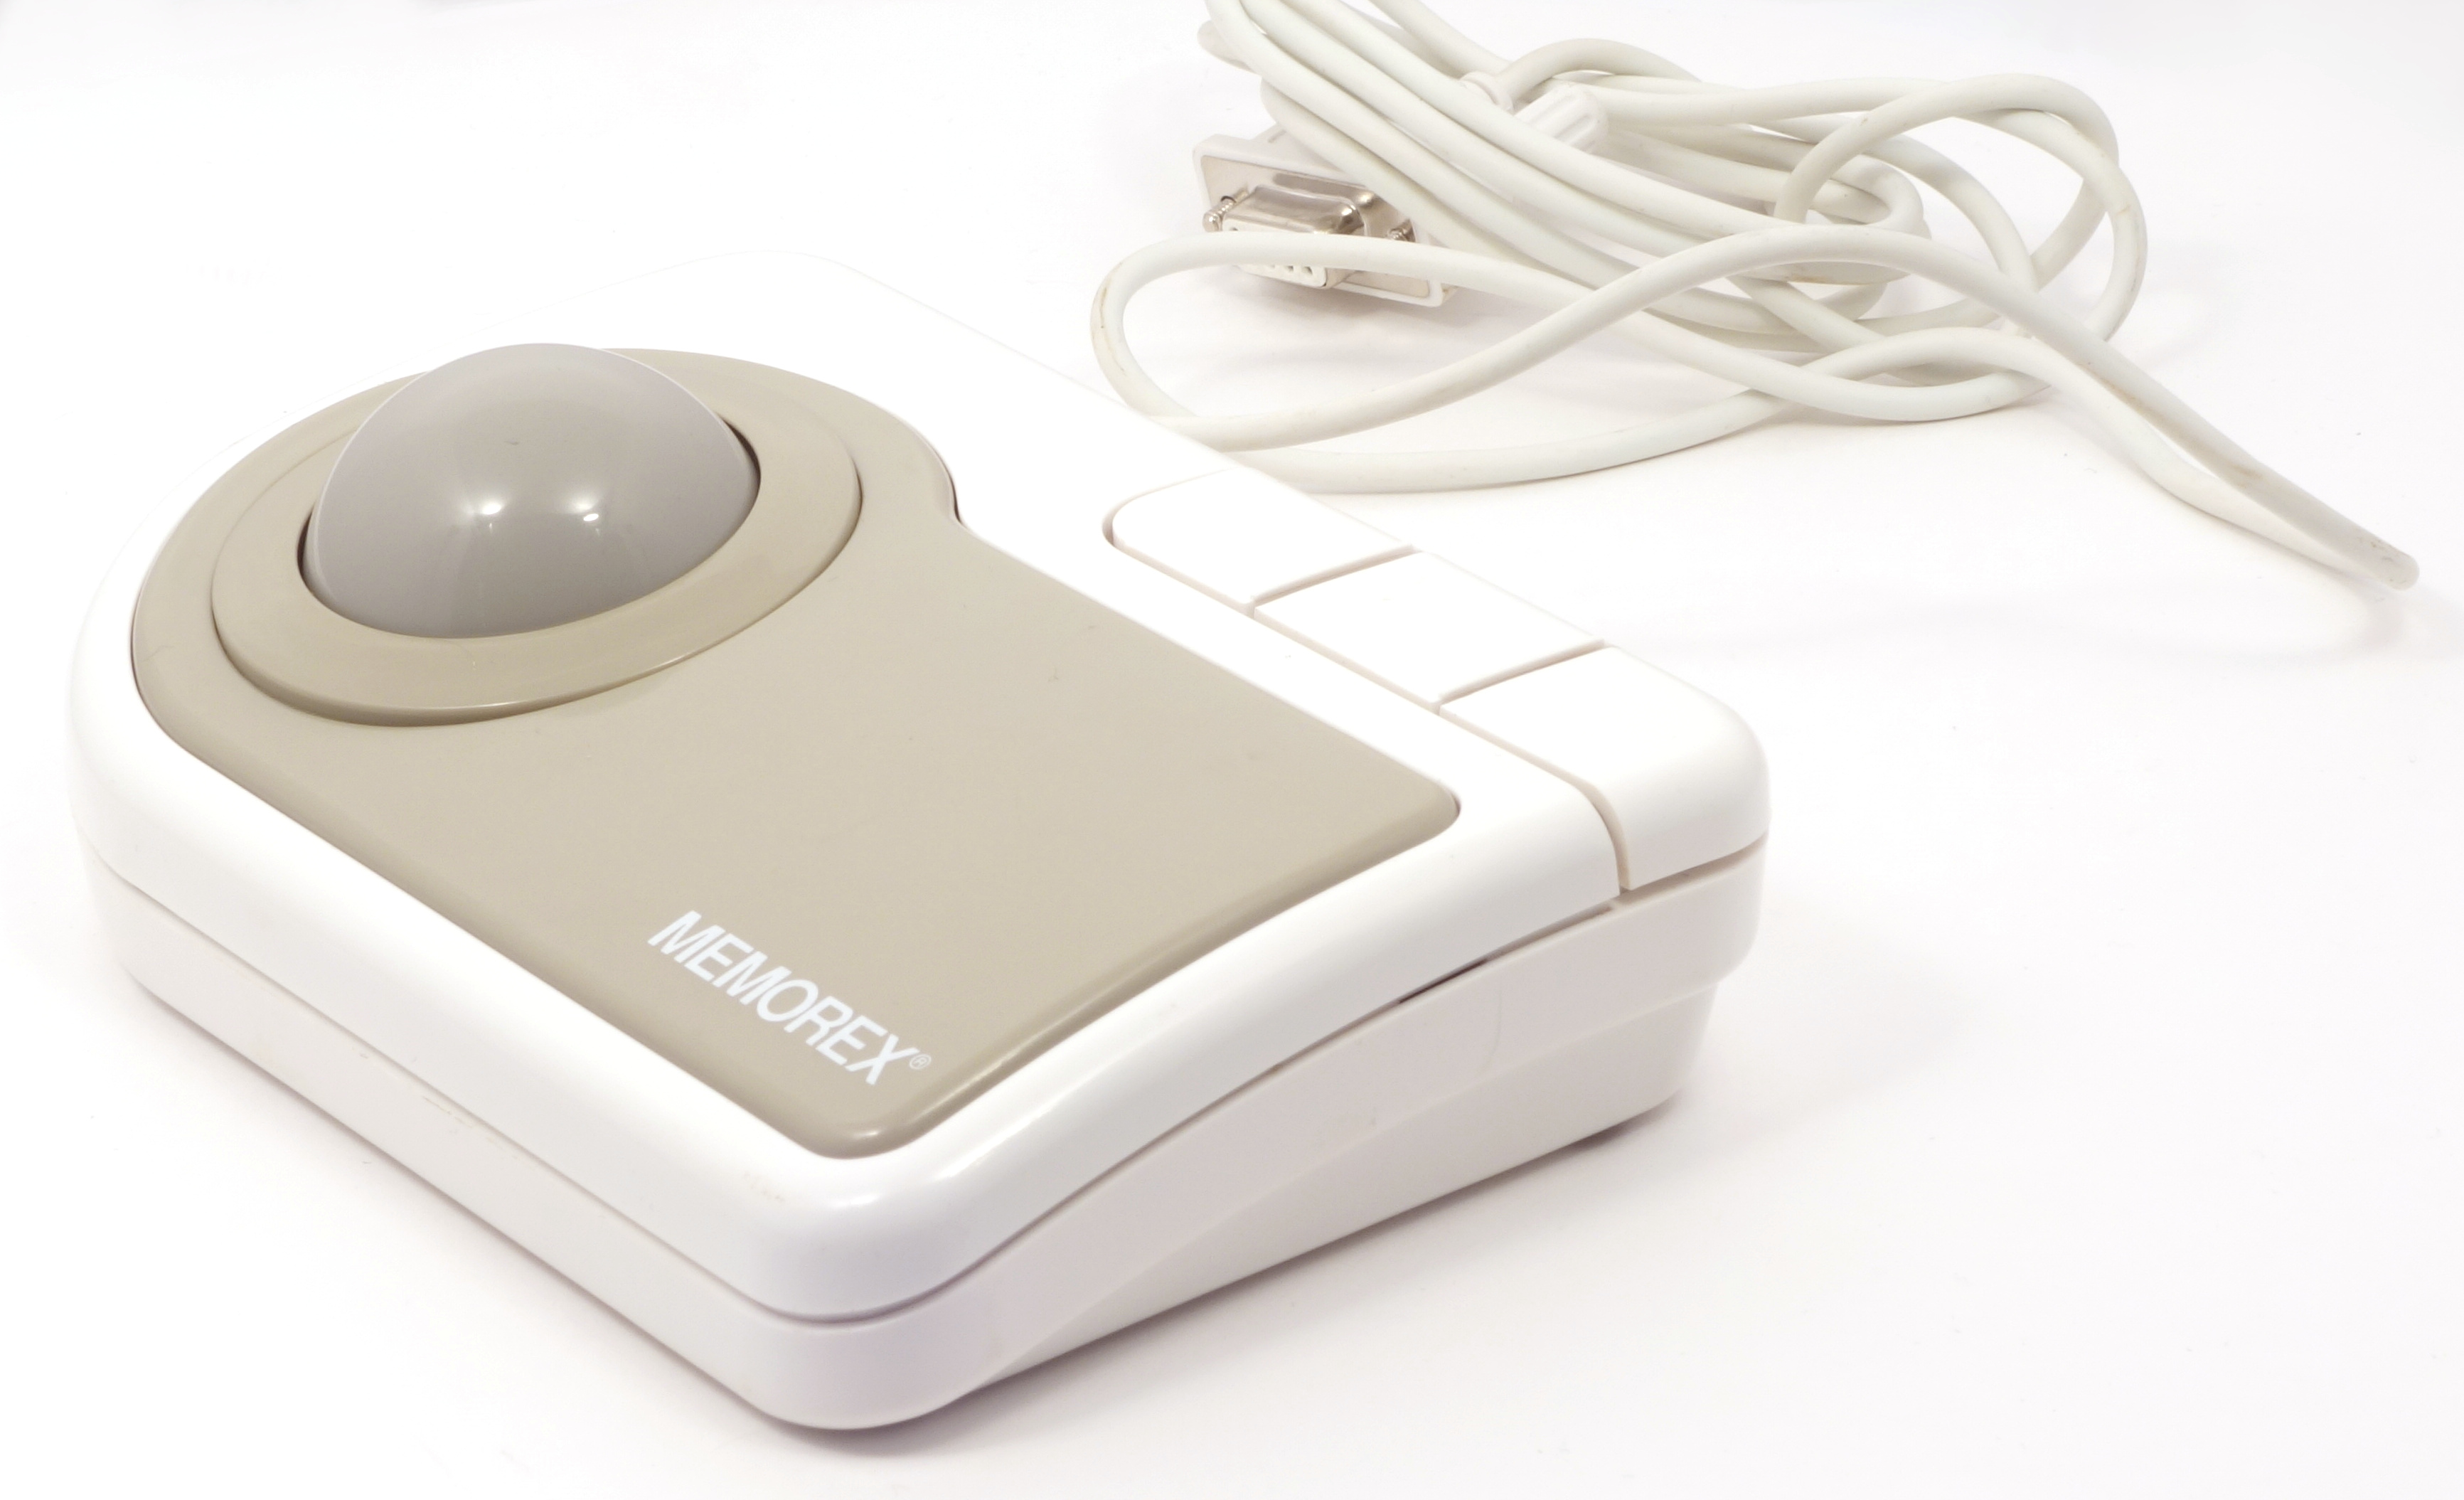
\includegraphics[scale=0.55]{1994_memorex_trackball/pic_30.jpg}
    \caption{Memorex trackball}
    \label{fig:MemorexPic}
\end{figure}

The body of the trackball is asymmetrical, made in a minimalist style of glossy white plastic with a brown insert.

\begin{figure}[h]
    \centering
    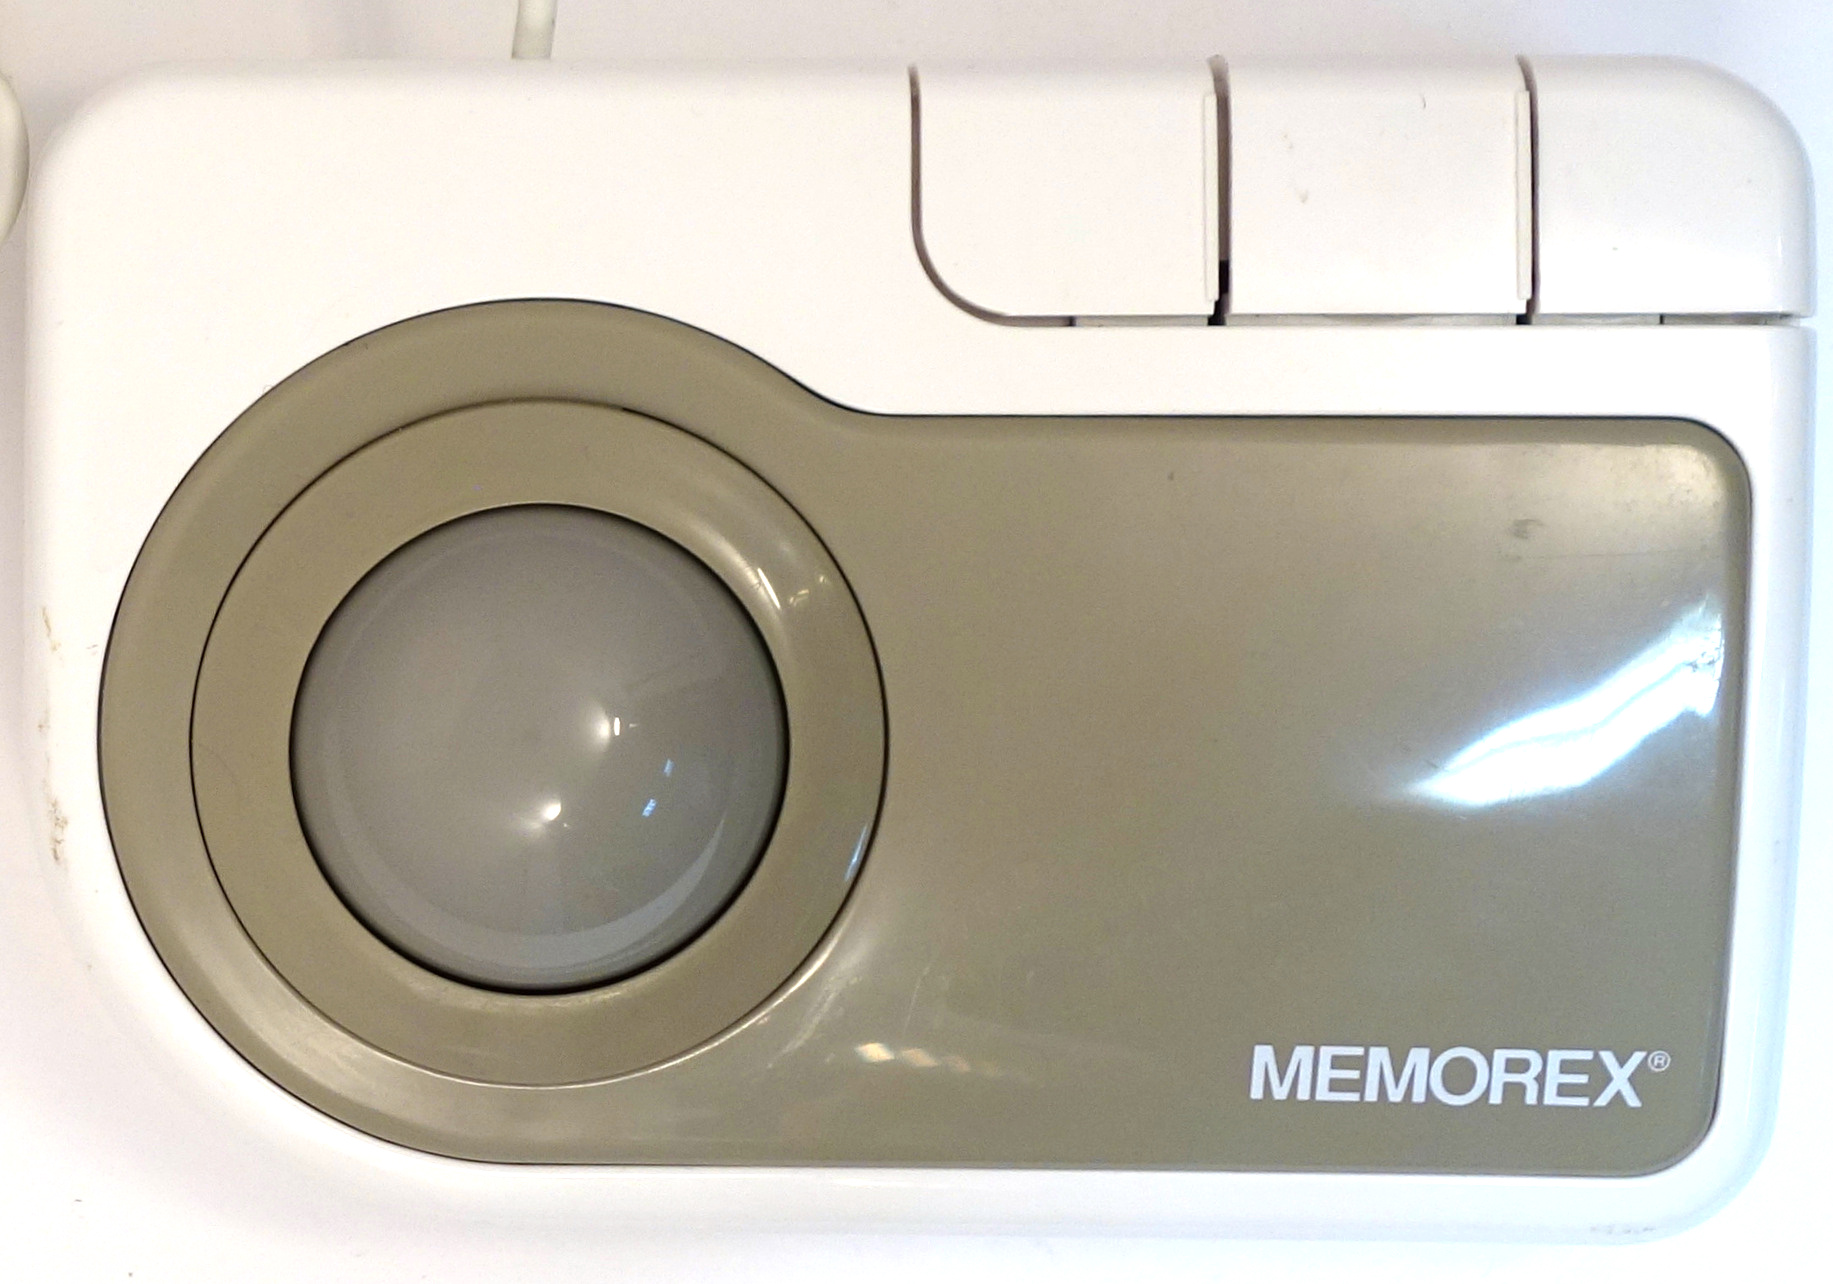
\includegraphics[scale=0.5]{1994_memorex_trackball/top_30.jpg}
    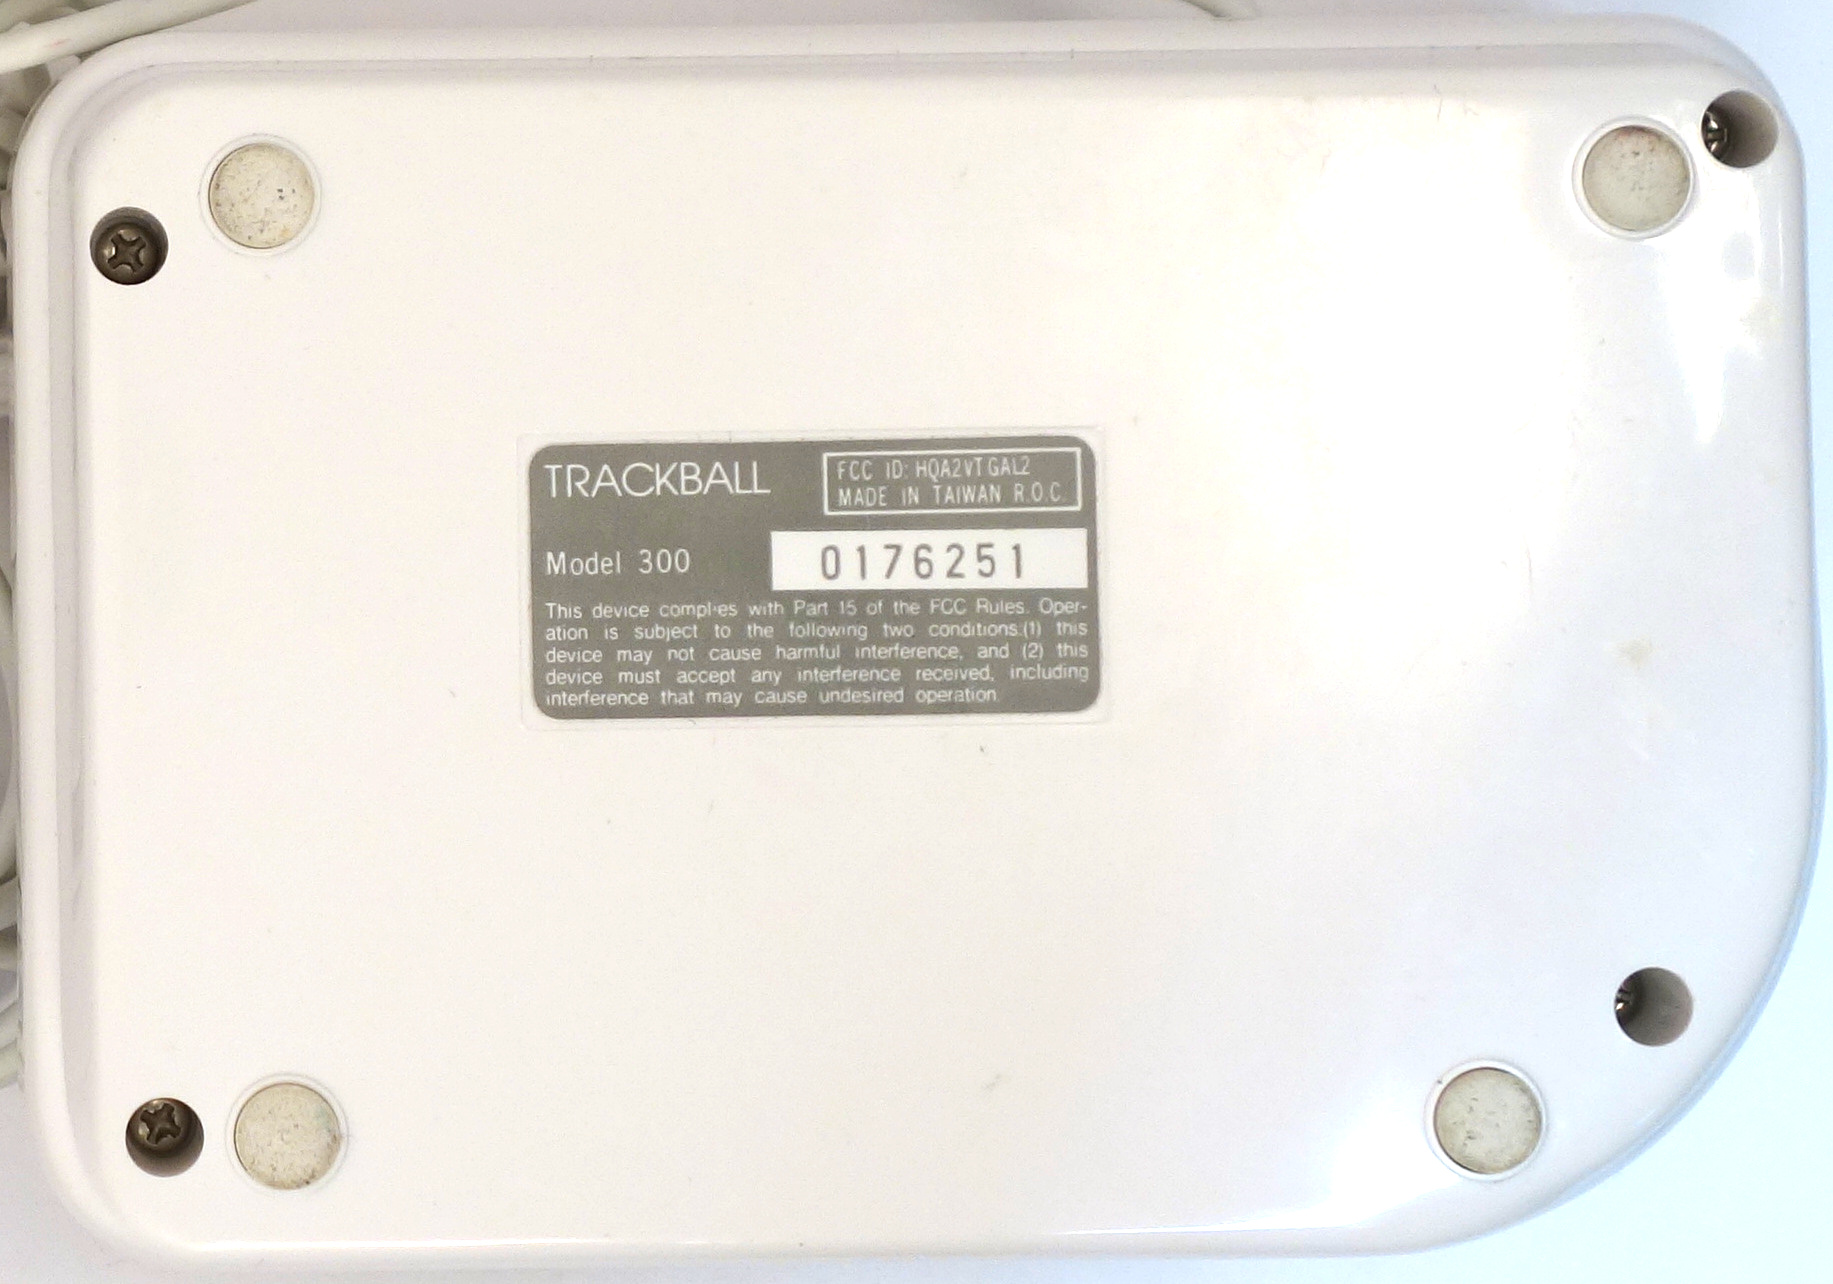
\includegraphics[scale=0.5]{1994_memorex_trackball/bottom_30.jpg}
    \caption{Memorex trackball, top and bottom views}
    \label{fig:MemorexTopBottom}
\end{figure}

As you can see in figure \ref{fig:MemorexSize}, this manipulator is relatively small.

The trackball packaging and user manual of the Memorex variant use the “Stationary Mouse” subtitle, apparently borrowed from the Logitech TrackMan Stationary Mouse trackball released a year earlier, and emphasize its ease of use in a limited workspace.

\begin{figure}[h]
    \centering
    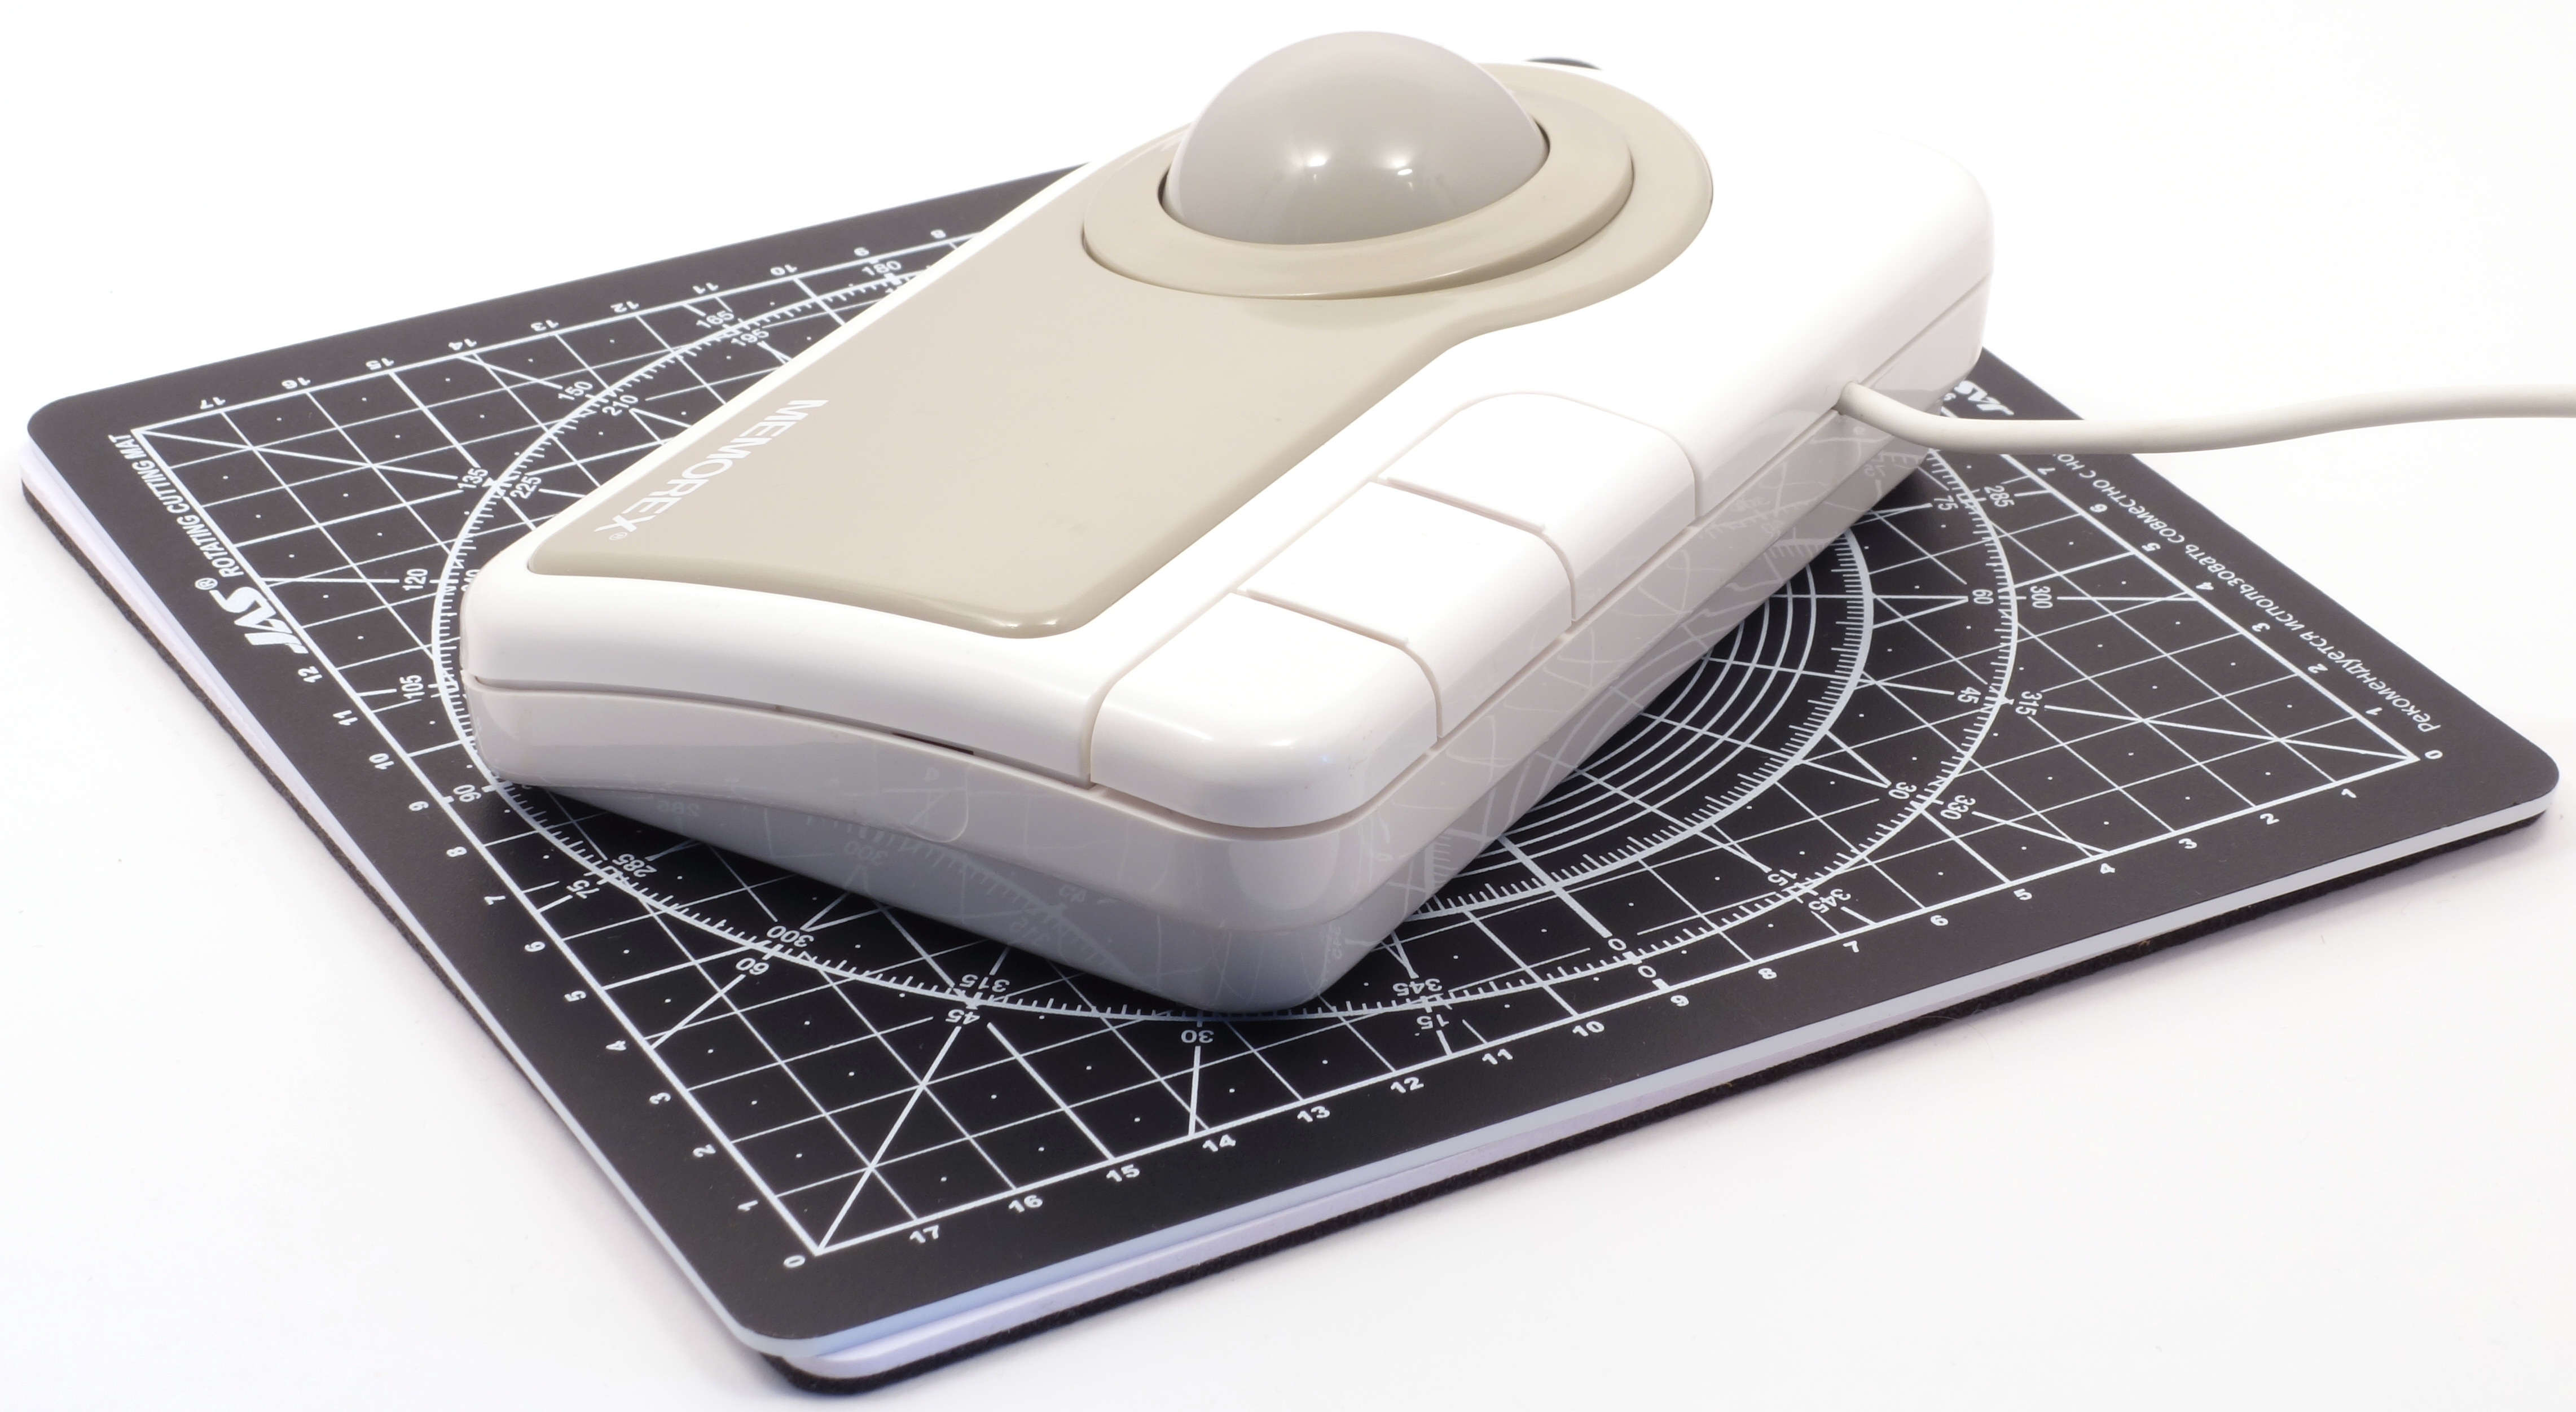
\includegraphics[scale=0.41]{1994_memorex_trackball/size_30.jpg}
    \caption{Memorex trackball on a graduated pad with a grid step of 1~cm}
    \label{fig:MemorexSize}
\end{figure}

The trackball is right-handed and the shape is largely inspired by the Logitech another product - LOGiTECH, which is also designed for a horizontal position of the hand and the rotation of the ball with the thumb (figure \ref{fig:MemorexHand}). According to Logitech, this shape is better suited to the anatomical structure of the hand (in advertising, the shape of classic symmetrical trackballs was opposed to a similar shape as a “device for aliens” \cite{adv}).

\begin{figure}[h]
    \centering
    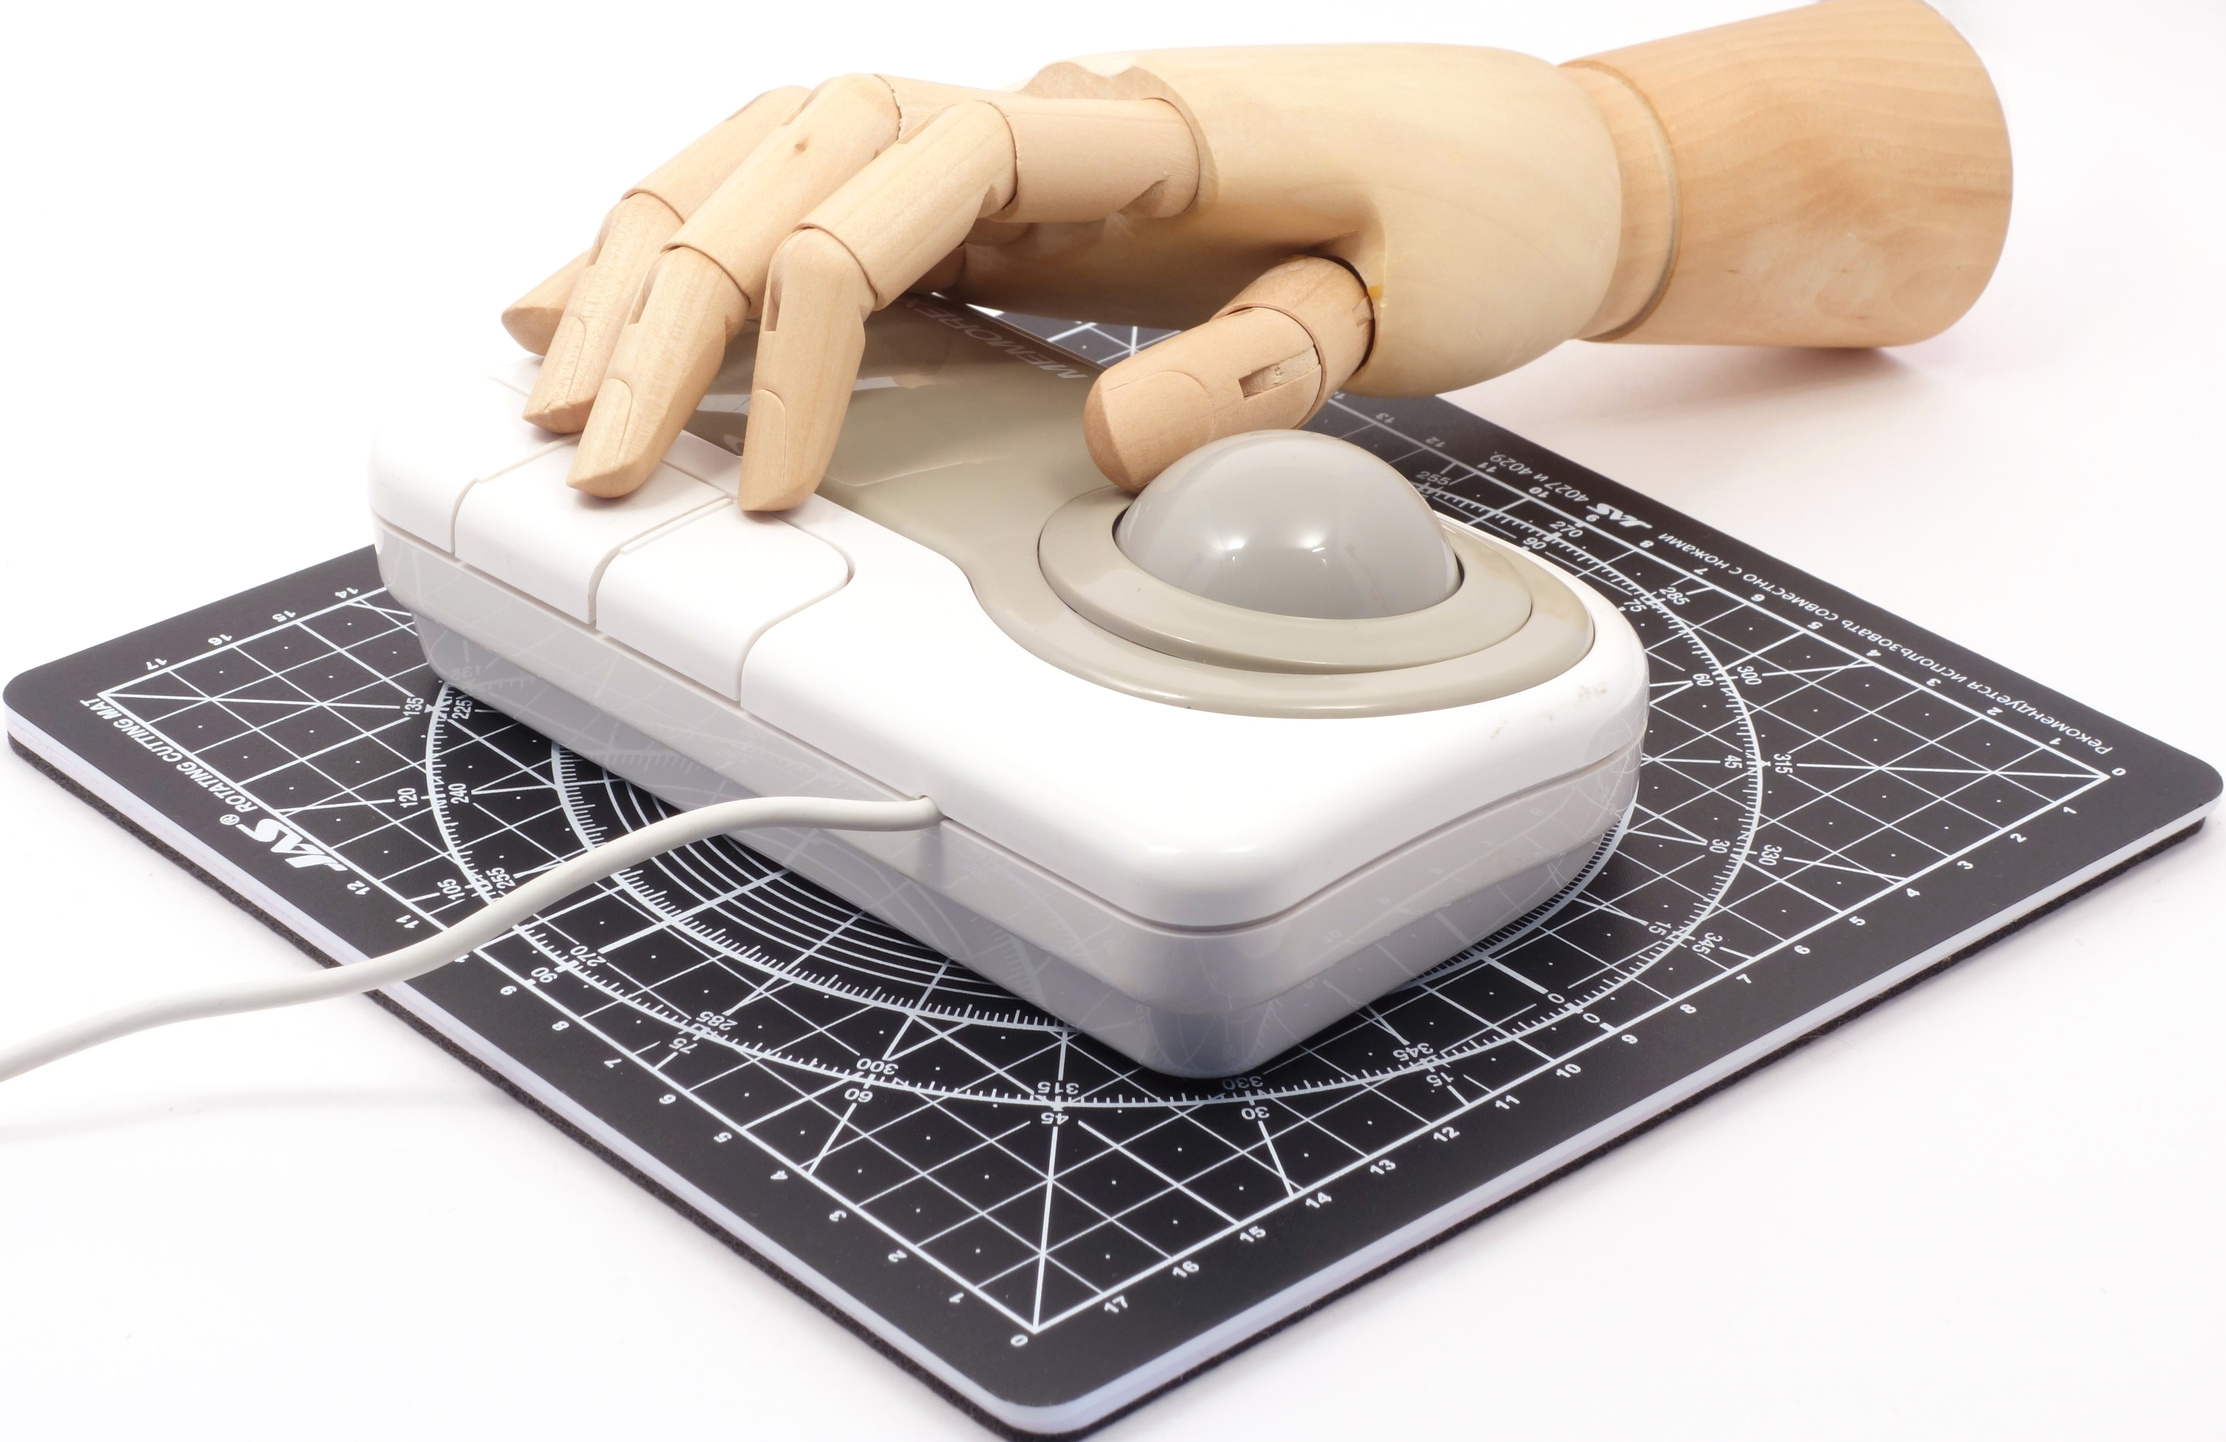
\includegraphics[scale=0.19]{1994_memorex_trackball/hand_30.jpg}
    \caption{Memorex trackball with a human hand model}
    \label{fig:MemorexHand}
\end{figure}

Trackball internals are shown on figure \ref{fig:MemorexInside}. It is an opto-mechanical device typical for the beginning of the 90s, in both the encoder implementation and the whole internal layout, which leaves a significant amount of empty space inside the case.

\begin{figure}[h]
    \centering
    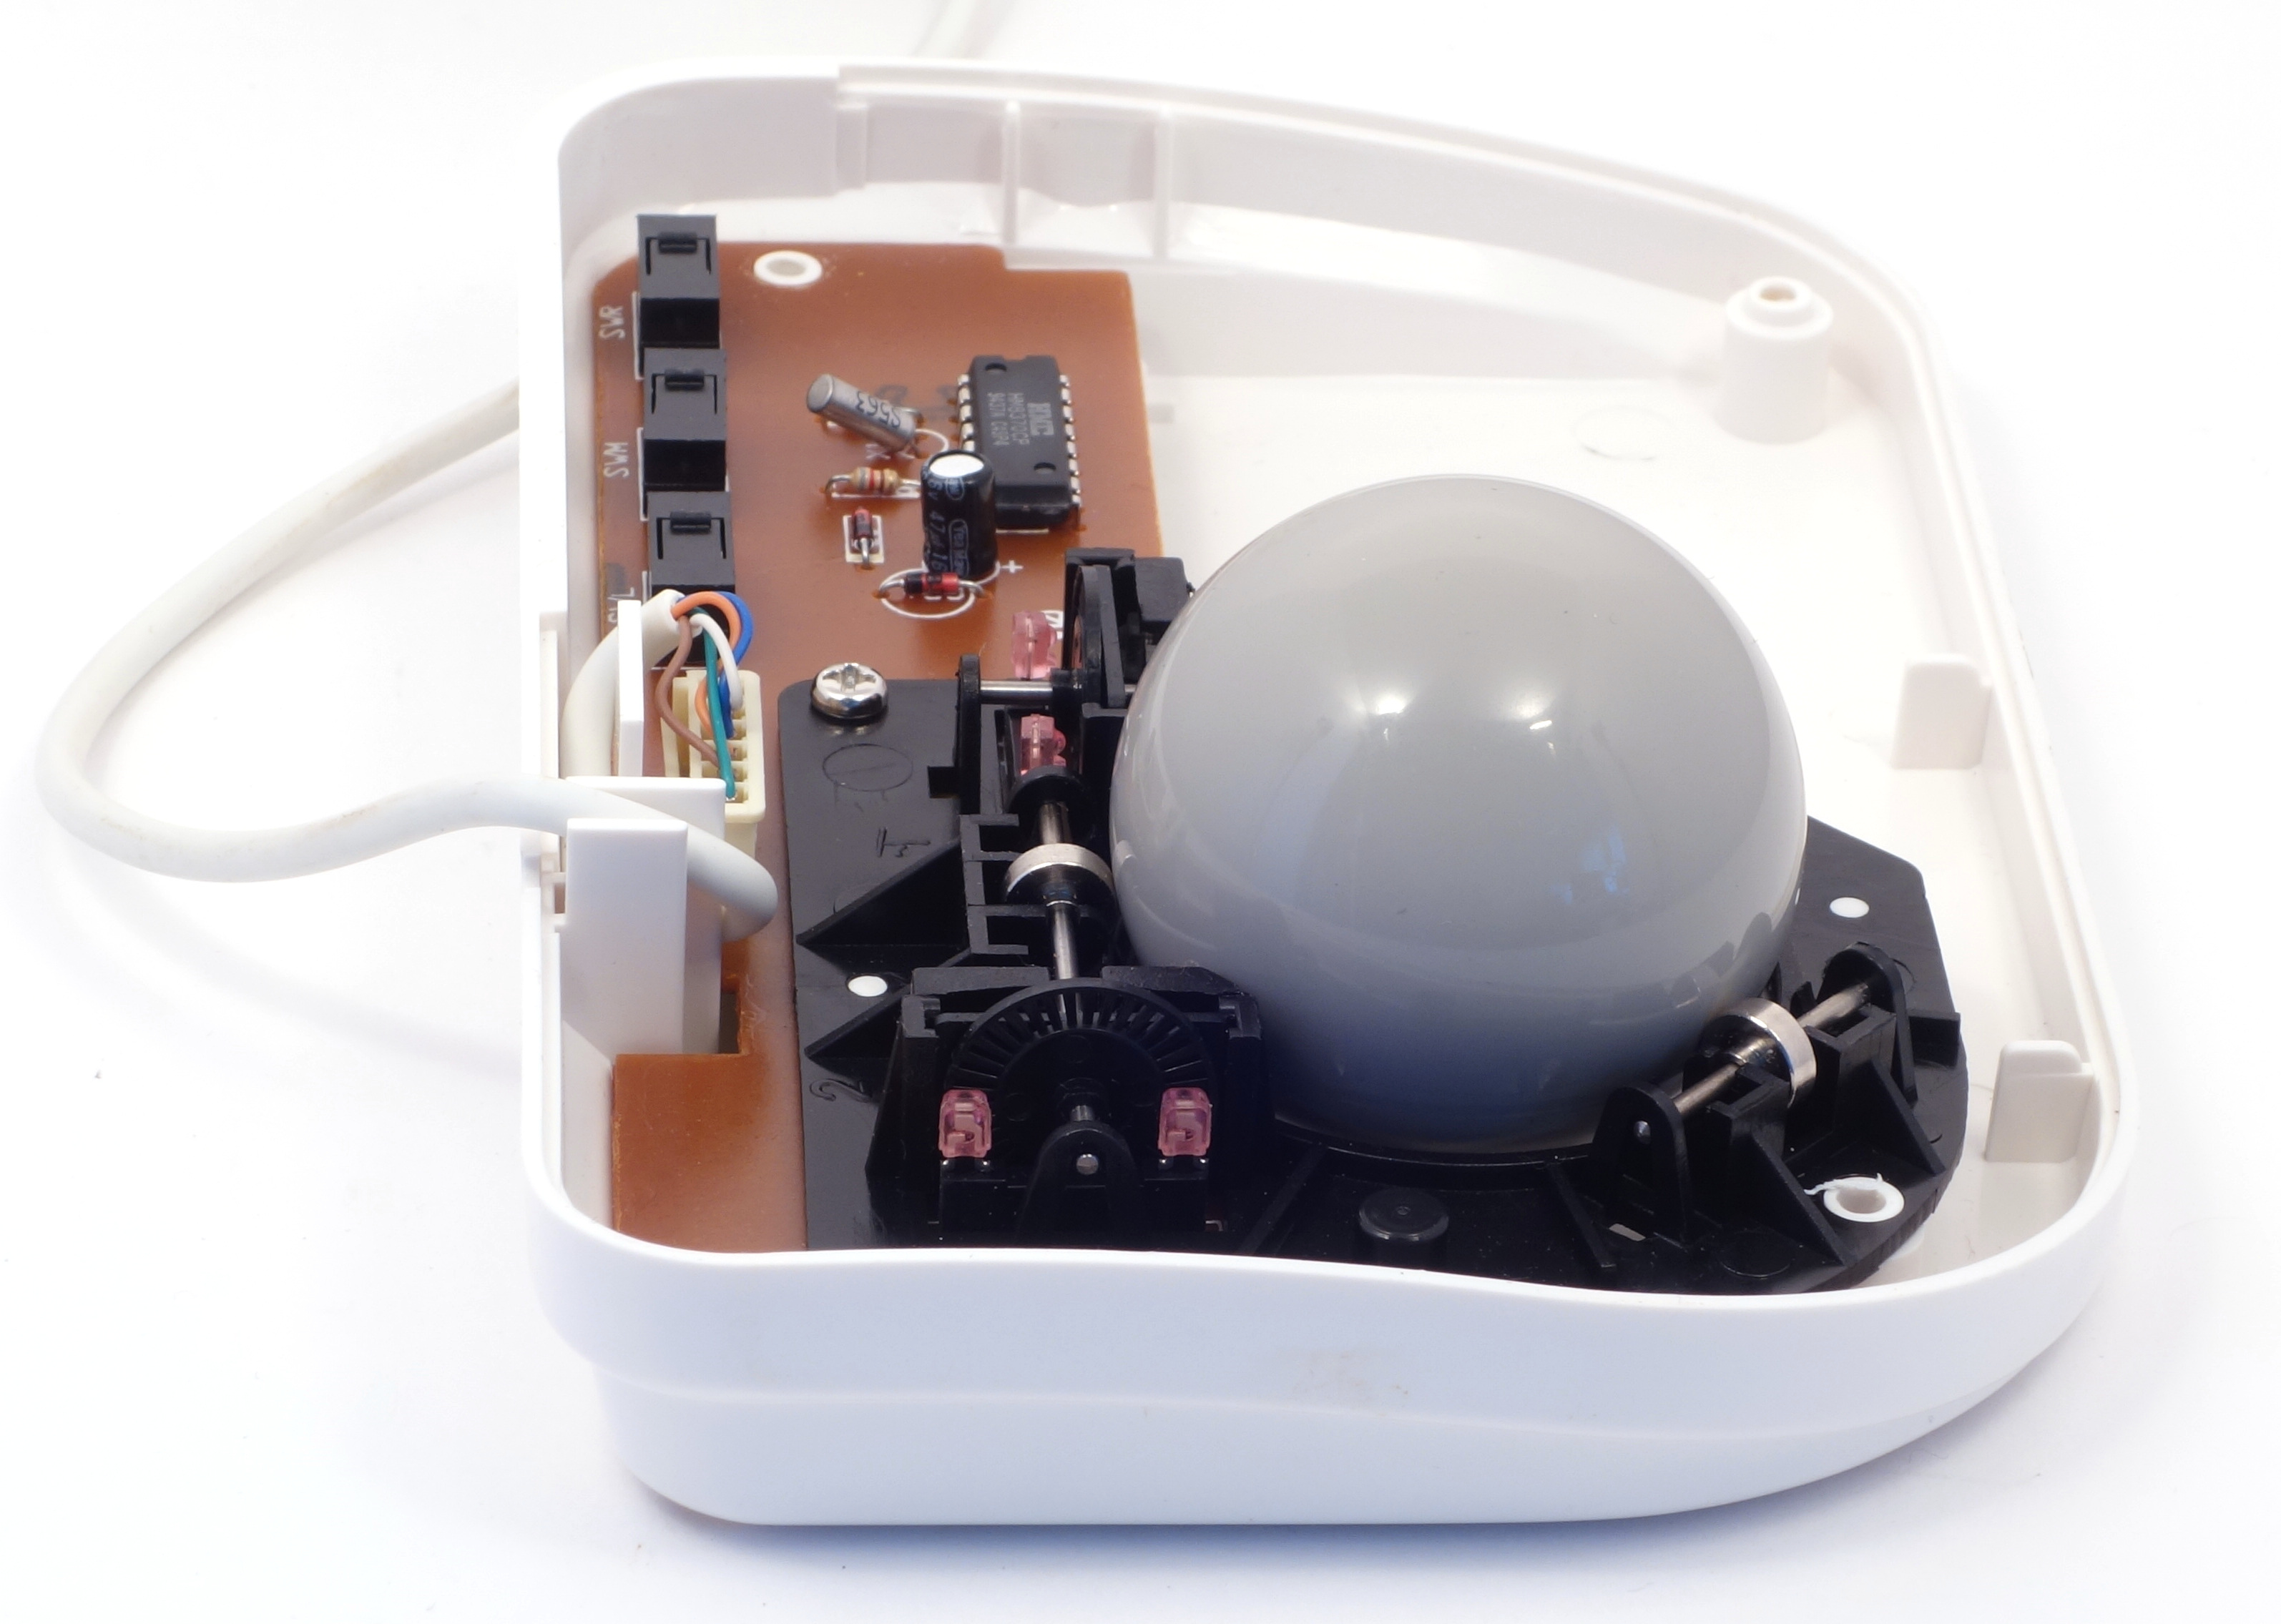
\includegraphics[scale=0.6]{1994_memorex_trackball/inside_30.jpg}
    \caption{Memorex trackball disassembled}
    \label{fig:MemorexInside}
\end{figure}

\begin{thebibliography}{9}
\bibitem {adv} Not every kind of pointing device fits your kind of hand (LOGiTECH TrackMan tadvertising). // PC Magazine. V.~8, No.~19. November, 1989, pp. 360-361. \url{https://archive.org/details/PC-Mag-1989-11-14/page/n361}
\end{thebibliography}
\end{document}
